\documentclass{article}
\usepackage[utf8]{inputenc}
\usepackage{amsmath,amssymb}
\usepackage{cancel}
\usepackage{makecell}
\usepackage[a4paper, total={6in, 9in}]{geometry}
\usepackage{authblk}
\usepackage{graphicx}
\graphicspath{{.}}
\author{Zihan Zhao}
\affil{1001103708}
\title{Homework 2}
\date{}
\begin{document}
\maketitle
\section{}
\renewcommand{\thesubsection}{(\alph{subsection})}
\subsection{}
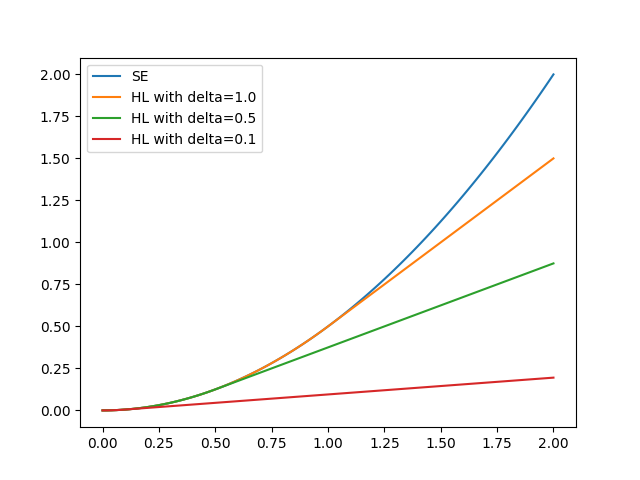
\includegraphics{q1a.png}
Compared with squared error loss, when the residue (y-t) increases, Huber loss is the same as squared error loss. But when it reaches over the threshold $\delta$, i.e. the loss is at outliers, Huber loss becomes linearly increasing by the slope of $\delta$. It becomes less sensitive to outliers than squared error loss. So the optimal weights can be determined more quickly by using Huber loss gradient descent. Moreover, as $\delta$ decreases, the loss is further away from squared error loss. The degree of insensitivity becomes larger. Therefore it is robust regression.
\subsection{}
Now determines $\frac{\mathrm{d} L_\delta}{\mathrm{d} w}$:
\begin{align*}
    \frac{\mathrm{d} L_\delta}{\mathrm{d} w}&=  \frac{\mathrm{d} H_\delta (a)}{\mathrm{d} a} \frac{\mathrm{d} a}{\mathrm{d} y}\frac{\mathrm{d} y}{\mathrm{d} w}\\
\intertext{When $|y-t| \leqq \delta$:}
    &= \frac{\mathrm{d} \frac{1}{2}a^2 }{\mathrm{d} a} \frac{\mathrm{d} a}{\mathrm{d} y} \frac{\mathrm{d} y}{\mathrm{d} w}\\
    &= a * 1 * x = ax = (y-t)x\\
    &= (w^\intercal x+b-t)x\\
\intertext{When $|y-t| > \delta$:}
    &= \frac{\mathrm{d} \delta(|a|-\frac{1}{2}\delta)}{\mathrm{d} a} \frac{\mathrm{d} a}{\mathrm{d} y} \frac{\mathrm{d} y}{\mathrm{d} w}\\
    &=
    \begin{cases}
    \delta x, &y-t>\delta\\
    -\delta x, &y-t<-\delta\\
    \end{cases}
\end{align*}
Now determines $\frac{\mathrm{d} L_\delta}{\mathrm{d} b}$:
\begin{align*}
    \frac{\mathrm{d} L_\delta}{\mathrm{d} b}&=  \frac{\mathrm{d} H_\delta (a)}{\mathrm{d} a} \frac{\mathrm{d} a}{\mathrm{d} y}\frac{\mathrm{d} y}{\mathrm{d} b}\\
\intertext{When $|y-t| \leqq \delta$:}
    &= \frac{\mathrm{d} \frac{1}{2}a^2 }{\mathrm{d} a} \frac{\mathrm{d} a}{\mathrm{d} y} \frac{\mathrm{d} y}{\mathrm{d} b}\\
    &= a * 1 * 1 = x\\
    &= w^\intercal x+b-t\\
\intertext{When $|y-t| > \delta$:}
    &= \frac{\mathrm{d} \delta(|a|-\frac{1}{2}\delta)}{\mathrm{d} a} \frac{\mathrm{d} a}{\mathrm{d} y} \frac{\mathrm{d} y}{\mathrm{d} w}\\
    &=
    \begin{cases}
    \delta , &y-t>\delta\\
    -\delta , &y-t<-\delta\\
    \end{cases}
\end{align*}
\subsection{}
Look at q1.py.
\section{}
\subsection{}
First factor the Loss formula:
\begin{align*}
    L &= \frac{1}{2}\sum_{i = 1}^{N} a^{(i)} (y^{(i)} - w^\intercal x^{(i)} )^2 + \frac{\lambda}{2}||w||^2 \\
    &= \frac{1}{2}A||Y-Xw||^2 + \frac{\lambda}{2}w^\intercal w \; \text{(where Y is Nx1, X is Nxd, A is NxN, and w is dx1)}\\
    &= \frac{1}{2}(Y-Xw)^\intercal (A(Y-Xw)) + \frac{\lambda}{2}w^\intercal w\\
    &= \frac{1}{2}(Y^\intercal AY-Y^\intercal AXw -(Xw)^\intercal AY + w^\intercal X^\intercal AXw) + \frac{\lambda}{2}w^\intercal w\\
    &= \frac{1}{2}(Y^\intercal AY-Y^\intercal AXw - (AY)^\intercal Xw + w^\intercal (X^\intercal AX)w) + \frac{\lambda}{2}w^\intercal w\\
    &= \frac{1}{2}(Y^\intercal AY-Y^\intercal AXw - Y^\intercal A^\intercal Xw + w^\intercal (X^\intercal AX)w) + \frac{\lambda}{2}w^\intercal w\\
\intertext{Since $A = A^\intercal$,}
    &= \frac{1}{2}(Y^\intercal AY-Y^\intercal AXw - Y^\intercal AXw + w^\intercal (X^\intercal AX)w) + \frac{\lambda}{2}w^\intercal w\\
    &= \frac{1}{2}Y^\intercal AY-Y^\intercal AXw + \frac{1}{2}w^\intercal (X^\intercal AX)w + \frac{\lambda}{2}w^\intercal w\\
\end{align*}
Now take derivative of L by w:
\begin{align*}
\intertext{Since $A = A^\intercal$, so $X^\intercal AX$ is symmatric as well, then}
    \frac{\mathrm{d} L}{\mathrm{d} w} &= 0-Y^\intercal AX + \frac{1}{2}2(X^\intercal AX)w + \frac{1}{2}2\lambda w\\
    &= -Y^\intercal AX  + (X^\intercal AX)w + \lambda w\\
\intertext{Let $\frac{\mathrm{d} L}{\mathrm{d} w} = 0$, we got}
-Y^\intercal AX  + (X^\intercal AX)w + \lambda w &= 0\\
(X^\intercal AX + \lambda I)w &= Y^\intercal AX\\
w &= (X^\intercal AX + \lambda I)^{-1}Y^\intercal AX\\
\intertext{Since $Y^\intercal AX = (AX)^\intercal Y = X^\intercal A^\intercal Y = X^\intercal A Y$,}
w &= (X^\intercal AX + \lambda I)^{-1}X^\intercal AY\\
\end{align*}
Done.
\subsection{}
Look at q2.py.
\subsection{}
Now take a look at the training error. When $\tau$ is small, the divergence among the elements in $A_{ii}$ gets large, the reweighted error loss will put larger weights on the data whose is far away from its target and put smaller weights on the data which is close to its target. So the optimmal weight will produce more precise prediction.  When $\tau$ is too large, $a^{(i)}$ approaches to the same value $\frac{1}{N}$. So the loss will put same weights on each data and cannot enlarge the error where data is far from its target. The training loss is larger than when $\tau$ is small.\\\\
Then take a look at the validation error. When $\tau$ is small, overfitting occurs. The reason is that when training the data, the gradient descent specifies each weight for each training data and enlarges the data weight as it is far from its target. It is overfitting. Then it causes the total loss of validation data to be higher. When $\tau$ becomes larger, weights of each data approaches to the same value, overfitting is reduced. Then validation error follows training error to increase.\\\\
Look at q2.py. The training loss and validation loss are shown in the following figure. My guess is similar with the figure.\\
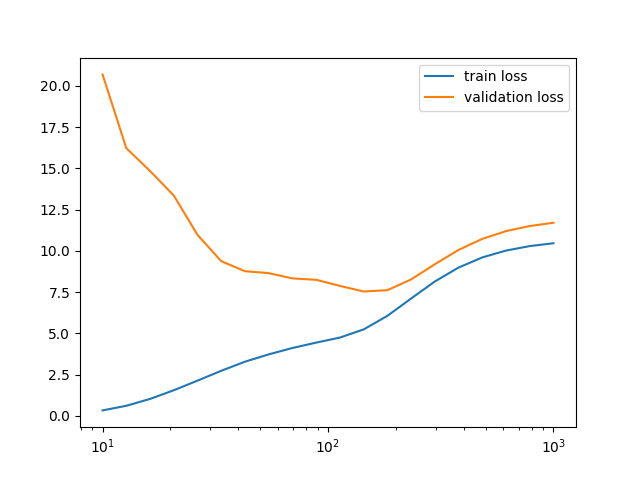
\includegraphics{q2c.png}
\section{}
Denote:
\begin{align*}
    LEFT\; SIDE &= err^\prime_t\\
                &= \frac{\sum_{i = 1}^{N}\omega ^\prime_i 1\{h_t(x^i)\neq t^i\}}{\sum_{i = 1}^{N}\omega ^\prime_i}\\
    RIGHT\; SIDE &= \frac{1}{2}\\
\intertext{Also from Tips}
    E &= \{i: h_t(x^i)\neq t^i\}\\
    E^c &= \{i: h_t(x^i) = t^i\}
\end{align*}
So we can pick all i whose $i\in E$ to rewrite LEFT SIDE:
\begin{align*}
    LEFT\; SIDE &= \frac{\sum_{i\in E}^{}\omega ^\prime_i}{\sum_{i = 1}^{N}\omega ^\prime_i}\\
\intertext{We know the updated weight $\omega ^\prime_i = \omega _ie^{-\alpha _t t^ih_t(x^i)}$, plug it in LEFT SIZE:}
    &= \frac{\sum_{i\in E}^{}\omega _ie^{-\alpha _t t^ih_t(x^i)}}{\sum_{i = 1}^{N}\omega ^\prime_i}\\
\intertext{In E, $t^i$ and $h_t(x^i)$ should be 1/-1 or -1/1, so $t^ih_t(x^i)=-1$. Then:}
    &= \frac{\sum_{i\in E}^{}\omega _ie^{\alpha _t}}{\sum_{i = 1}^{N}\omega ^\prime_i}\\
\intertext{Plug $\alpha _t = \frac{1}{2}\log \frac{1-err_t}{err_t}$ in LEFT SIZE:}
    &= \frac{\sum_{i\in E}^{}\omega _ie^{\frac{1}{2}\log \frac{1-err_t}{err_t}}}{\sum_{i = 1}^{N}\omega ^\prime_i}\\
    &= \frac{\sum_{i\in E}^{}\omega _i(\frac{1-err_t}{err_t})^{\frac{1}{2}}}{\sum_{i = 1}^{N}\omega ^\prime_i}\\
\intertext{The denominator is converted in the same way. Notice in $E^c$, $t^ih_t(x^i)=1$,}
    &= \frac{\sum_{i\in E}^{}\omega _i(\frac{1-err_t}{err_t})^{\frac{1}{2}}}{\sum_{i = 1}^{E}\omega ^\prime_i + \sum_{j = 1}^{E^c}\omega ^\prime_j}\\
    &= \frac{\sum_{i\in E}^{}\omega _i(\frac{1-err_t}{err_t})^{\frac{1}{2}}}{\sum_{i\in E}^{}\omega _ie^{\frac{1}{2}\log \frac{1-err_t}{err_t}} + \sum_{j\in E^c}^{}\omega _je^{-\frac{1}{2}\log \frac{1-err_t}{err_t}}}\\
    &= \frac{\sum_{i\in E}^{}\omega _i(\frac{1-err_t}{err_t})^{\frac{1}{2}}}{\sum_{i\in E}^{}\omega _i(\frac{1-err_t}{err_t})^{\frac{1}{2}} + \sum_{j\in E^c}^{}\omega _j(\frac{1-err_t}{err_t})^{-\frac{1}{2}}}\\
    &= \frac{(\frac{1-err_t}{err_t})^{\frac{1}{2}}\sum_{i\in E}^{}\omega _i}{(\frac{1-err_t}{err_t})^{\frac{1}{2}}\sum_{i\in E}^{}\omega _i + (\frac{1-err_t}{err_t})^{-\frac{1}{2}}\sum_{j\in E^c}^{}\omega _j}\\
    &= \frac{\sum_{i\in E}^{}\omega _i}{\sum_{i\in E}^{}\omega _i + (\frac{1-err_t}{err_t})^{-1}\sum_{j\in E^c}^{}\omega _j}\\
\intertext{$err_t$ is the similar as $err^\prime_t$, that is $err_t = \frac{\sum_{i\in E}^{}\omega _i}{\sum_{i = 1}^{N}\omega _i}$. Then,}
    &= \frac{\sum_{i\in E}^{}\omega _i}{\sum_{i\in E}^{}\omega _i + (\frac{1-\frac{\sum_{i\in E}^{}\omega _i}{\sum_{i = 1}^{N}\omega _i}}{\frac{\sum_{i\in E}^{}\omega _i}{\sum_{i = 1}^{N}\omega _i}})^{-1}\sum_{j\in E^c}^{}\omega _j}\\
    &= \frac{\sum_{i\in E}^{}\omega _i}{\sum_{i\in E}^{}\omega _i + (\frac{\sum_{i = 1}^{N}\omega _i-\sum_{i\in E}^{}\omega _i}{\sum_{i\in E}^{}\omega _i})^{-1}\sum_{j\in E^c}^{}\omega _j}\\
    &= \frac{\sum_{i\in E}^{}\omega _i}{\sum_{i\in E}^{}\omega _i + (\frac{\sum_{i\in E}^{}\omega _i}{\sum_{i = 1}^{N}\omega _i-\sum_{i\in E}^{}\omega _i})\sum_{j\in E^c}^{}\omega _j}\\
    &= \frac{\sum_{i\in E}^{}\omega _i}{\sum_{i\in E}^{}\omega _i + \frac{\sum_{i\in E}^{}\omega _i}{\sum_{j\in E^c}^{}\omega _j}\sum_{j\in E^c}^{}\omega _j}\\
    &= \frac{\sum_{i\in E}^{}\omega _i}{\sum_{i\in E}^{}\omega _i + \frac{\sum_{i\in E}^{}\omega _i}{\cancel{\sum_{j\in E^c}^{}\omega _j}}\cancel{\sum_{j\in E^c}^{}\omega _j}}\\
    &= \frac{\sum_{i\in E}^{}\omega _i}{2\sum_{i\in E}^{}\omega _i}\\
    &= \frac{1}{2} = RIGHT\; SIDE\\
\end{align*}
Done.
\end{document}
